\chapter{Metodolog\'ia}

\label{Chapter3}

En este cap\'itulo se detallar\'an los procesos abordados para la extracci\'on y clasificaci\'on de los d\'igitos
escritos en los telegramas de las elecciones.

\section{Extracci\'on, transformaci\'on y carga de d\'igitos de los telegramas}

Los telegramas de las elecciones de Santa Fe presentan un formato tabular, donde cada fila representa un partido
pol\'itico y los votos obtenidos abiertos por senadores y diputados. Se debieron ejecutar m\'ultiples pasos de
extracci\'on, transformaci\'on y carga (ETL por sus siglas) de los mismos antes de poder armar un dataset con el cual
entrenar los modelos. Se utiliz\'o la librer\'ia OpenCV \parencite{opencv_library} para manipular las im\'agenes y poder llevar a cabo el proceso de ETL.

\subsection{Enderezado}
Como los telegramas son escaneados a mano, el primer paso consiste en enderezarlos. Este proceso puede realizarse
buscando el rect\'angulo de mayor \'area, calculando el \'angulo de rotaci\'on y rotando la imagen completa con la
funci\'on \verb|getRotationMatrix2D| de OpenCV.

\begin{figure}[H]
    \centering

    \tikzset{every picture/.style={line width=0.75pt}}

    \begin{tikzpicture}[x=0.75pt,y=0.75pt,yscale=-1,xscale=1]

        \draw (370,140) node  {\includegraphics[width=135pt,height=210pt]{chapter3/etl-2-rotacion.png}};
        \draw (90,140) node  {\includegraphics[width=135pt,height=210pt]{chapter3/etl-1-telegrama.png}};
        \draw    (190.8,110.6) -- (267.4,110.6) ;
        \draw [shift={(269.4,110.6)}, rotate = 180] [color={rgb, 255:red, 0; green, 0; blue, 0 }  ][line width=0.75]    (10.93,-3.29) .. controls (6.95,-1.4) and (3.31,-0.3) .. (0,0) .. controls (3.31,0.3) and (6.95,1.4) .. (10.93,3.29)   ;
        \draw (190,87.18) node [anchor=north west][inner sep=0.75pt]   [align=left] {Enderezar};

    \end{tikzpicture}

    \caption{Enderezamiento de un telegrama utilizando OpenCV.}
    \label{fig:etl-1-rotacion}
\end{figure}

\subsection{Extracci\'on de la grilla de votos}
El siguiente paso consiste en poder seleccionar la grilla de los votos y poder extraerla para seguir trabajando en
ella.

\section{Dise\~{n}o experimental}

\lipsum[1]

\section{M\'etricas de evaluaci\'on}

Los modelos entrenados ser\'an evaluados con distintas m\'etricas, descripta en las siguientes sub-secciones del
cap\'itulo. Las mismas pretenden evaluar qu\'e tan buenos son los modelos y qu\'e capacidad de adaptaci\'on de dominio
poseen.

\subsection{Accuracy}

La m\'etrica de {\it accuracy} permite identificar qu\'e tan cerca o lejos un conjunto de observaciones se encuentra
respecto a los valores reales. Es el ratio de predicciones correctas sobre las totales.

\begin{equation}
    Accuracy(y, \hat{y}) = \frac{1}{n} \sum_{i=0}^{n-1} 1(\hat{y_{i}}=y_{i})
\end{equation}

Donde:
\begin{itemize}
    \item $n$: es la cantidad de observaciones totales.
    \item $y_{i}$: es el valor de la ${i}$-\'esima observaci\'on correspondiente al real.
    \item $\hat{y_{i}}$: es el valor predicho para la ${i}$-\'esima observaci\'on.
    \item $1(x)$: es la funci\'on indicador.
\end{itemize}

\subsection{$F_{1}$}

La m\'etrica $F_{1}$ es una media arm\'onica de otras dos: {\it precisi\'on} y {\it recall}. De manera simplificada, la
primera muestra la capacidad del modelo de no etiquetar como positivo una obsevaci\'on que es negativa y la segunda
muestra la capacidad del modelo de encontrar todas las observaciones positivas.

La {\it precisi\'on} consiste en calcular el ratio de predicciones positivas correctas de la clase respecto al total de
predicciones positivas de la clase.

\begin{equation}
    Precision(y, \hat{y}) = \frac{TP}{TP + FP}
\end{equation}

Donde:
\begin{itemize}
    \item $TP$: es la cantidad de verdaderos positivos.
    \item $FP$: es la cantidad de falsos positivos.
\end{itemize}

Por otro lado, el {\it recall} consiste en calcular el ratio de predicciones positivas correctas de la clase respecto
al total de predicciones correctas de la clase.

\begin{equation}
    Recall(y, \hat{y}) = \frac{TP}{TP + FN}
\end{equation}

Donde:
\begin{itemize}
    \item $TP$: es la cantidad de verdaderos positivos.
    \item $FN$: es la cantidad de falsos negativos.
\end{itemize}

Las dos m\'etricas mencionada anteriormente pueden ser combinadas en una sola denominada $F_{\beta}$. El valor de
$\beta$ permite asignar un peso distinto a la precisi\'on o al recall dentro del promedio arm\'onico. Cuando $\beta=1$,
ambas poseen el mismo peso.

\begin{equation}
    F_{\beta}(y, \hat{y}) = (1 + \beta^2) \frac{precision(y, \hat{y}) \times recall(y, \hat{y})}{\beta^2 precision(y, \hat{y}) + recall(y, \hat{y})}
\end{equation}

El rango de valores es de $[0, 1]$, donde 1 corresponde a un clasificador que funciona sin errores.

\subsection{Intersecci\'on sobre uni\'on}

Otra forma de medir el clasificador es mediante la {\it intersecci\'on sobre uni\'on} (IoU por sus siglas en ingl\'es).
Consta de calcular la cantidad de d\'igitos \'unicos predichos por sobre la cantidad de d\'igitos \'unicos reales. Por
ejemplo, para un telegrama y un partido el clasificador predice 189 votos cuando lo real es 180. Entonces, el {\it IoU}
viene dado por:

\begin{align}
    IoU(\{1, 8, 0\}, \{1, 8, 9\}) & = \frac{\lvert\{1, 8, 0\} \bigcap \{1, 8, 9\}\rvert}{\lvert\{1, 8, 0\} \bigcup \{1, 8, 9\}\rvert} \nonumber \\
                                  & = \frac{\lvert\{1, 8\}\rvert}{\lvert\{1, 8, 0, 9\}\rvert}                                         \nonumber \\
                                  & = \frac{2}{4}                                                                     \nonumber                 \\
                                  & = 0.5
\end{align}

De forma general: sea $y_{i}$ el d\'igito $i$-\'esimo del voto real $y$, $\hat{y_{i}}$ el d\'igito $i$-\'esimo del voto
predicho por el modelo $\hat{y}$, entonces la m\'etrica viene dada por:

\begin{equation}
    IoU(y, \hat{y}) = \frac{\lvert \{y_{i}\} \bigcap \{\hat{y_{i}}\}\rvert}{\lvert \{y_{i}\} \bigcup \{\hat{y_{i}}\}\rvert}
\end{equation}

\subsection{Distancia $\mathcal{A}$}

La distancia $\mathcal{A}$ mide la similaridad entre dos distribuciones. Puede ser utilizada para analizar los espacios
latentes de clasificadores en problemas de adaptaci\'on de dominio \parencite{ben2006analysis}. La m\'etrica viene dada por:

\begin{equation}
    dist_\mathcal{A} = 2 (1-2\epsilon)
\end{equation}

Donde $\epsilon$ es el error en test de un clasificador entrenado para discriminar el dominio de origen del de destino.
Cuando el error de clasificaci\'on es bajo, significa que hay diferencias significativas entre las dos distrubiones,
haciendo que $dist_\mathcal{A}$ sea grande y vice versa.

En la figura \ref{fig:ejemplos-dist-a} se muestran posibles casos de distribuciones de dominios. En la sub-figura
\ref{fig:dominios-distintos} las distribuciones de dominios son significativamente diferentes entre si, por lo tanto
$dist_\mathcal{A} \approx 2$. Por el contrario, en la sub-figura \ref{fig:dominios-similares} las distribuciones de
dominios son similares entre si, por lo que se espera que $dist_\mathcal{A} \approx 0$.

\begin{figure}[H]
    \centering
    \begin{subfigure}[h]{0.46\textwidth}
        \centering
        \tikzset{every picture/.style={line width=0.75pt}}
        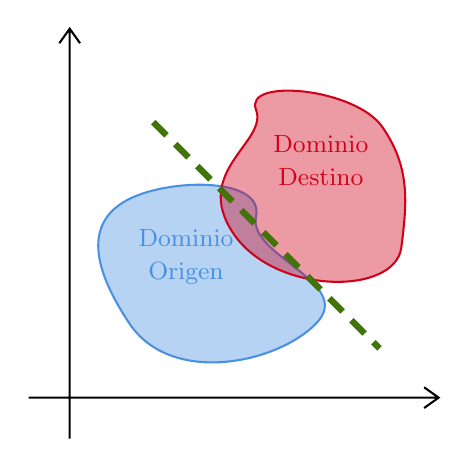
\begin{tikzpicture}[x=0.75pt,y=0.75pt,yscale=-1,xscale=1]
            \draw  (0,177.75) -- (197.5,177.75)(19.75,0) -- (19.75,197.5) (190.5,172.75) -- (197.5,177.75) -- (190.5,182.75) (14.75,7) -- (19.75,0) -- (24.75,7)  ;
            \draw  [color={rgb, 255:red, 74; green, 144; blue, 226 }  ,draw opacity=1 ][fill={rgb, 255:red, 74; green, 144; blue, 226 }  ,fill opacity=0.4 ] (48.5,82) .. controls (68.5,72) and (113.5,71.5) .. (109.5,90.5) .. controls (105.5,109.5) and (157.5,122.5) .. (138.5,142) .. controls (119.5,161.5) and (68.5,172) .. (48.5,142) .. controls (28.5,112) and (28.5,92) .. (48.5,82) -- cycle ;
            \draw  [color={rgb, 255:red, 208; green, 2; blue, 27 }  ,draw opacity=1 ][fill={rgb, 255:red, 208; green, 2; blue, 27 }  ,fill opacity=0.4 ] (109.5,39) .. controls (103.5,23.5) and (157.5,28.5) .. (170.5,47.5) .. controls (183.5,66.5) and (182.5,82.5) .. (179.5,105.5) .. controls (176.5,128.5) and (118.5,128.5) .. (98.5,98.5) .. controls (78.5,68.5) and (115.5,54.5) .. (109.5,39) -- cycle ;
            \draw (115,50) node [anchor=north west][inner sep=0.75pt]  [color={rgb, 255:red, 208; green, 2; blue, 27 }  ,opacity=1 ] [align=left] {\begin{minipage}[lt]{36.4pt}\setlength\topsep{0pt}
                    \begin{center}
                        {\small Dominio}\\{\small Destino}
                    \end{center}

                \end{minipage}};
            \draw (50,95) node [anchor=north west][inner sep=0.75pt]  [color={rgb, 255:red, 74; green, 144; blue, 226 }  ,opacity=1 ] [align=left] {\begin{minipage}[lt]{36.4pt}\setlength\topsep{0pt}
                    \begin{center}
                        {\small Dominio}\\{\small Origen}
                    \end{center}

                \end{minipage}};
            \draw [color={rgb, 255:red, 65; green, 117; blue, 5 }  ,draw opacity=1 ][line width=2.25]  [dash pattern={on 6.75pt off 4.5pt}]  (60,45) -- (169,154) ;
        \end{tikzpicture}
        \caption{Dominios distintos, f\'acilmente discriminables.}
        \label{fig:dominios-distintos}
    \end{subfigure}
    \hfill
    \begin{subfigure}[h]{0.46\textwidth}
        \centering
        \tikzset{every picture/.style={line width=0.75pt}}

        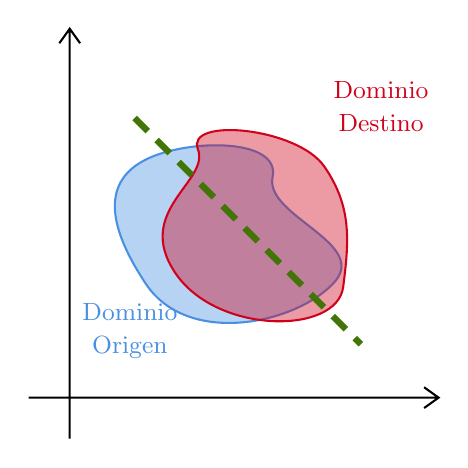
\begin{tikzpicture}[x=0.75pt,y=0.75pt,yscale=-1,xscale=1]
            \draw  (1,179.75) -- (198.5,179.75)(20.75,2) -- (20.75,199.5) (191.5,174.75) -- (198.5,179.75) -- (191.5,184.75) (15.75,9) -- (20.75,2) -- (25.75,9)  ;
            \draw  [color={rgb, 255:red, 74; green, 144; blue, 226 }  ,draw opacity=1 ][fill={rgb, 255:red, 74; green, 144; blue, 226 }  ,fill opacity=0.4 ] (57.5,65) .. controls (77.5,55) and (122.5,54.5) .. (118.5,73.5) .. controls (114.5,92.5) and (166.5,105.5) .. (147.5,125) .. controls (128.5,144.5) and (77.5,155) .. (57.5,125) .. controls (37.5,95) and (37.5,75) .. (57.5,65) -- cycle ;
            \draw  [color={rgb, 255:red, 208; green, 2; blue, 27 }  ,draw opacity=1 ][fill={rgb, 255:red, 208; green, 2; blue, 27 }  ,fill opacity=0.4 ] (82.5,60) .. controls (76.5,44.5) and (130.5,49.5) .. (143.5,68.5) .. controls (156.5,87.5) and (155.5,103.5) .. (152.5,126.5) .. controls (149.5,149.5) and (91.5,149.5) .. (71.5,119.5) .. controls (51.5,89.5) and (88.5,75.5) .. (82.5,60) -- cycle ;
            \draw [color={rgb, 255:red, 65; green, 117; blue, 5 }  ,draw opacity=1 ][line width=2.25]  [dash pattern={on 6.75pt off 4.5pt}]  (52,45) -- (161,154) ;

            \draw (24,133) node [anchor=north west][inner sep=0.75pt]  [color={rgb, 255:red, 74; green, 144; blue, 226 }  ,opacity=1 ] [align=left] {\begin{minipage}[lt]{36.4pt}\setlength\topsep{0pt}
                    \begin{center}
                        {\small Dominio}\\{\small Origen}
                    \end{center}

                \end{minipage}};
            \draw (145,26) node [anchor=north west][inner sep=0.75pt]  [color={rgb, 255:red, 208; green, 2; blue, 27 }  ,opacity=1 ] [align=left] {\begin{minipage}[lt]{36.4pt}\setlength\topsep{0pt}
                    \begin{center}
                        {\small Dominio}\\{\small Destino}
                    \end{center}

                \end{minipage}};
        \end{tikzpicture}

        \caption{Dominios similares, no discriminables.}
        \label{fig:dominios-similares}
    \end{subfigure}

    \caption{Ejemplos de distribuciones de dominios.}
    \label{fig:ejemplos-dist-a}
\end{figure}

Durante el proyecto se utiliza como clasificador una red de una capa densa con una funci\'on de activaci\'on sigmoidea,
es decir, una regresi\'on log\'istica.